In the following, $a||b$ denotes concatenation of strings $a$ and $b$.
$a{[i]}$ references the $i$-th byte in $a$. $(N,e)$ denotes an RSA public
key, where $N$ has byte-length $\ell_m$ ($|N|=\ell_m$) and $e$ is the public
exponent. The corresponding secret exponent is $d = 1/e \bmod \phi(N)$.

\subsection{\PKCS encryption padding}
\label{sec:PKCSdescr}

Our attacks rely on the structure of RSA \PKCS padding. Although RSA PKCS\#1
v2.0 implements OAEP, SSL/TLS still uses \PKCS. The \PKCS encryption padding
scheme~\cite{rfc2313} randomizes encryptions by prepending a random padding
string $PS$ to a message $k$ (here, a symmetric session key) before RSA
encryption:

\begin{enumerate} 
	\item The plaintext message is $k$, $\ell_k = |k|$. The encrypter generates a random byte
	string $PS$, where $|PS| \geq 8$, $|PS|=\ell_m-3-\ell_k$, and $\hex{00} \not \in \{PS{[1]}, \ldots,PS{[|PS|]}\}$. 
	\item The encryption block is $m = 00||02||PS||00||k$. 
	\item The ciphertext is computed as $c = m^e \bmod N$. 
\end{enumerate} 

To decrypt such a ciphertext, the decrypter first computes $m = c^d
\bmod N$.  Then it checks whether the decrypted message $m$ is
correctly formatted as a \PKCS-encoded message. We say that the
ciphertext $c$ and the decrypted message bytes $m{[1]} || m{[2]} || ... ||
m{[\ell_m]}$ are \PKCSconform if:
\begin{equation*} 
	\begin{split} 
		m{[1]}||m{[2]} \text{ } = &\text{ } \hex{00} || \hex{02}\\
		\hex{00} \text{ } \not \in &\text{ } \{m{[3]}, \ldots,m{[10]}\}\\ 
	\end{split}
\end{equation*} 
If this condition holds, the decrypter searches for the first value
$i>10$ such that $m{[i]}=0x00$. Then, it extracts $k =
m{[i+1]}||\ldots||m{[\ell_m]}$. Otherwise, the ciphertext is rejected.

In SSLv3 and TLS, RSA \PKCS is used to encapsulate the \pms exchanged during
the handshake~\cite{rfc5246}. Thus, $k$ is interpreted as the \pms. In SSLv2,
RSA \PKCS is used for encapsulation of an equivalent key denoted the
\texttt{master\_key}.


\subsection{SSL and TLS}
The first incarnation of the TLS protocol was the SSL (Secure Socket Layer)
protocol, which was designed by Netscape in the 90s. The first two versions
of SSL were immediately found to be vulnerable to trivial
attacks~\cite{rfc6176,ssl-v3-1996} which were fixed in SSLv3~\cite{rfc6101}.
Later versions of the standard were renamed TLS, and share a similar
structure to SSLv3. The current version of the protocol is TLS 1.2; TLS 1.3
is currently under development.

An SSL/TLS protocol flow consists of two phases: handshake and
application data exchange. In the first phase, the communicating
parties agree on cryptographic algorithms and establish shared
keys. In the second phase, these keys are used to protect the
confidentiality and authenticity of the transmitted application data.

The handshake protocol was fundamentally redesigned in the \sslthree
version. This new handshake protocol was then used in later TLS
versions up to TLS 1.2. In the following, we describe the RSA-based
handshake protocols used in TLS and \ssltwo, and highlight their
differences.

\paragraph{The \ssltwo handshake protocol.}
\label{sec:ssl2}

The \ssltwo protocol description~\cite{sslv2} is less formally specified than
modern RFCs. Figure~\ref{fig:ssl-handshake} depicts an \ssltwo handshake.

\begin{figure}
	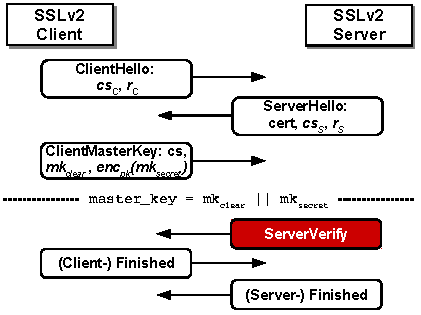
\includegraphics[width=\linewidth]{\DrownFigures/ssl-handshake} 
	\caption{\textbf{\ssltwo handshake}\,---\,%
	The server responds with a \texttt{ServerVerify} message directly after
    receiving an RSA-\PKCS ciphertext contained in \texttt{ClientMasterKey}.
	This protocol feature enables the attack.
	}
	\label{fig:ssl-handshake}
\end{figure}

A client initiates an \ssltwo handshake by sending a
\texttt{ClientHello} message, which includes a list of cipher
suites $cs_c$ supported by the client and a client nonce $r_c$,
termed \texttt{challenge}.
The server responds with a \texttt{ServerHello} message, which
contains a list of cipher suites $cs_s$ supported by the server,
the server certificate, and a server nonce $r_s$, termed
$\texttt{connection\_ID}$.

The client responds with a \texttt{ClientMasterKey} message, which
specifies a cipher suite supported by both peers and key data
used for constructing a \texttt{master\_key}. In order to support
\textit{export} cipher suites with 40-bit security (e.g.,
\texttt{SSL\_RC2\_128\_CBC\_EXPORT40\_WITH\_MD5}), the key data is
divided into two parts:
\begin{itemize}
	\item $mk_{clear}$: A portion of the \texttt{master\_key} sent in the \texttt{ClientMasterKey} message as plaintext (termed \texttt{clear\_key\_data} in the \ssltwo standard).
	\item $mk_{secret}$: A secret portion of the
          \texttt{master\_key}, encrypted with RSA \PKCS (termed \texttt{secret\_key\_data}). 
\end{itemize}
The resulting \texttt{master\_key} $mk$ is constructed by
concatenating these two keys: $mk = mk_{clear} || mk_{secret}$. For
40-bit export cipher suites, $mk_{secret}$ is five bytes in length.
For non-export cipher suites, the whole \texttt{master\_key} is
encrypted, and the length of $mk_{clear}$ is zero.

The client and server can then compute session keys from the reconstructed \texttt{master\_key} $mk$:

\vspace{-6pt}
\begin{center}
\begin{math}
	\texttt{server\_write\_key} = MD5(mk || ``0" || r_c || r_s) \linebreak	
	\texttt{client\_write\_key} = MD5(mk || ``1" || r_c || r_s)
\end{math}
\end{center}
\vspace{-6pt}

The server responds with a \texttt{ServerVerify} message
consisting of the \texttt{challenge} $r_c$ encrypted with the
\texttt{server\_write\_key}.  Both peers then exchange
\texttt{Finished} messages in order to authenticate to each other.

Our attack exploits the fact that the server always decrypts an RSA-\PKCS
ciphertext, computes the \texttt{server\_write\_key}, and \textit{immediately}
responds with a \texttt{ServerVerify} message.  The \ssltwo standard
implies this message ordering, but does not make it explicit.
However, we observed this behavior in every implementation we
examined.  Our attack also takes advantage of the fact that the
encrypted $mk_{secret}$ portion of the \texttt{master\_key} can vary
in length, and is only five bytes for export ciphers.

\ifsubmit\relax\else
\begin{figure}
	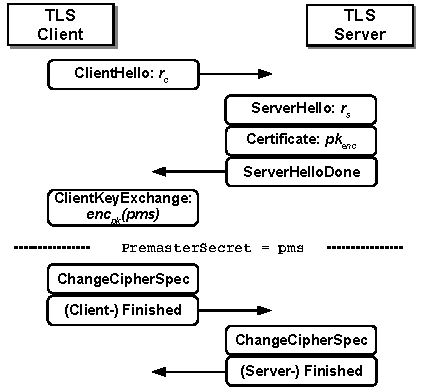
\includegraphics[width=\linewidth]{\DrownFigures/tls-handshake} 
	\caption{\textbf{TLS-RSA handshake}\,---\,%
    After receiving an encrypted \pms, the server waits for an authenticated
	\texttt{ClientFinished} message.
	}
	\label{fig:tls-handshake}
\end{figure}
\fi

\paragraph{The TLS handshake protocol.}
In TLS~\cite{rfc5246} or \sslthree, the client initiates the handshake with a \texttt{ClientHello}, which contains a client random $r_c$ and a list of supported cipher suites. The server chooses one of the cipher suites and responds with three messages, \texttt{ServerHello}, \texttt{Certificate}, and \texttt{ServerHelloDone}. These messages include the server's choice of cipher suite, server nonce $r_s$, and a server certificate with an RSA public key. The client then uses the public key to encrypt a newly generated 48-byte \pms $pms$ and sends it to the server in a \texttt{ClientKeyExchange} message. The client and server then derive encryption and MAC keys from the \pms and the client and server random nonces. The details of this derivation are not important to our attack.  The client then sends \texttt{ChangeCipherSpec} and \texttt{Finished} messages. The \texttt{Finished} message authenticates all previous handshake messages using the derived keys. The server responds with its own \texttt{ChangeCipherSpec} and \texttt{Finished} messages.

The two main details relevant to our attacks are:
\begin{itemize}
	\item The \pms is always 48 bytes long, independent of the chosen cipher suite.  This is also true for export cipher suites.
	\item After receiving the \texttt{ClientKeyExchange} message, the server waits for the \texttt{ClientFinished} message, in order to authenticate the client.
\end{itemize}


\subsubsection{Real-world protocol support}
TLSv1.0 is the most commonly supported protocol version, according to several
surveys. The SSL Labs SSL Pulse survey~\cite{ssl-pulse} reports that 98.6\%
of about 140,000 popular TLS/SSL-enabled web sites supported TLSv1.0 in
January 2016. 72.0\% supported TLSv1.2. Support for \ssltwo was at 9.3\%, and
\sslthree was at 29\%. Mayer et al.~\cite{mail-tls-mayer-2015} performed
Internet-wide surveys of SMTP, IMAP, and POP3 between April and August 2015,
and found that support for \ssltwo support was as high as 41.7\% of servers
for SMTP on port 25 and as low as 3.7\% of IMAP servers on port 143. Support
for TLSv1.0 was nearly universal on these ports, varying from 91.6\% on port
25 to 98.9\% on port 143.

Bowen~\cite{cab-forum-sslv2} collected 213 million SSL/TLS client hellos and
user agent strings from connections to popular sites, of which 183,000
(0.09\%) client hellos supported \ssltwo. All of these client hellos also
supported at least TLSv1.0.

Holz et al.~\cite{mail-tls-holz-2016} performed passive monitoring to collect
information about 16 million SSL/TLS connections during one week in
July-August 2015. They did not report any numbers for \ssltwo, and stated in
personal communication that they did not observe any \ssltwo connections in
their dataset.

%In response to our disclosure, OpenSSL has disabled \ssltwo by default in the 1.0.1r and 1.0.2f releases~\cite{opensslchangelog}.  

%This bug was also fixed in the aforementioned openssl releases.

\subsection{Bleichenbacher's attack}
\label{sec:bleichenbacher}
Bleichenbacher's attack is a padding oracle attack---it exploits the fact
that RSA ciphertexts should decrypt to \PKCS-compliant plaintexts. If an
implementation receives an RSA ciphertext that decrypts to an invalid \PKCS
plaintext, it might naturally leak this information via an error message, by
closing the connection, or by taking longer to process the error condition.
This behavior can leak information about the plaintext that can be modeled as
a cryptographic \textit{oracle} for the decryption process.
Bleichenbacher~\cite{bleichenbacher-1998} demonstrated how such an oracle
could be exploited to decrypt RSA ciphertexts.

%For example, the decrypting code may require different processing times for valid vs.\ invalid plaintexts - this is termed a "timing side-channel vulnerability". As another example, the decrypting code may send messages derived in some way from the plaintexts - this is termed a "direct message side channel vulnerability".
%The seminal work in this area \cite{Bleichenbacher} identified the general potential for such vulnerabilities, specifically using a direct message side channel vulnerability present in TLS implementations at the time, and demonstrated how such information could be gradually combined to eventually decrypt the RSA ciphertext in full.

\paragraph{Algorithm.}
In the simplest attack scenario, the attacker has a valid \PKCS
ciphertext $c_{0}$ that they wish to decrypt to discover the message
$m_{0}$.  They have no access to the private RSA key, but instead have
access to an oracle $\Oracle$ that will decrypt a ciphertext $c$ and
inform the attacker whether the most significant two bytes match
the required value for a correct \PKCS padding:
\begin{equation*} 
\Oracle(c) =  
\begin{cases} 
1 & \text{ if } m=c^d \bmod N \text{ starts with \hexb{00}{02}} \\ 
0 & \text{ otherwise.} 
\end{cases} 
\end{equation*} 

If the oracle answers with \texttt{1}, the attacker knows that $2B
\leq m \leq 3B-1$, where $B = 2^{8(\ell_m-2)}$.  The attacker can
take advantage of RSA malleability to generate new candidate ciphertexts
for any $s$:
\[
c = (c_{0} \cdot s^e) \bmod N = (m_{0} \cdot s)^e \bmod N 
\]
The attacker queries the oracle with $c$. If the oracle responds with
$0$, the attacker increments $s$ and repeats the previous
step. Otherwise, the attacker learns that for some~$r$, $2B \leq m_{0}s - rN  < 3B$. This allows the attacker to reduce the range of possible solutions to:  
\[ 
\frac{2B+rN}{s} \leq m_{0} < \frac{3B+rN}{s}  
\] 
The attacker proceeds by refining guesses for $s$ and $r$ values and
successively decreasing the size of the interval containing $m_{0}$.  At
some point the interval will contain a single valid value, $m_{0}$.
Bleichenbacher's original paper describes this process in further
detail~\cite{bleichenbacher-1998}.

\paragraph{Countermeasures.}
In order to protect against this attack, the decrypter must not leak
information about the \PKCS validity of the ciphertext.  The
ciphertext does not decrypt to a valid message, so the
decrypter generates a fake plaintext and continues the
protocol with this decoy.  The attacker should not be able to
distinguish the resulting computation from a correctly decrypted
ciphertext.

In the case of SSL/TLS, the server generates a random \pms to continue
the handshake if the decrypted ciphertext is
invalid.  The client will not possess the session key to send a valid
\texttt{ClientFinished} message and the connection will terminate.

